\documentclass{article}
\usepackage[utf8]{inputenc}
\usepackage{graphicx}
\usepackage{amsmath}

\title{Homework Set 10 - PHYS 728 Radio Astronomy}
\author{Matthew Cooper}
\date{April 19th, 2019}
\begin{document}
\begin{titlepage}
\maketitle
\end{titlepage}

\textbf{Problem 10.1-Solution}:  

\smallskip
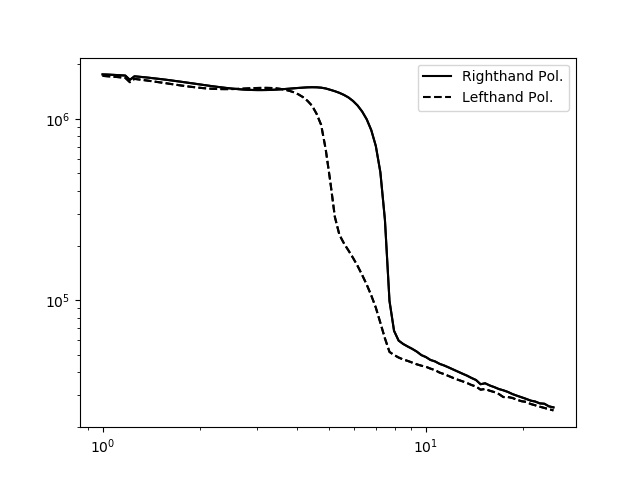
\includegraphics[scale=.7]{/home/matthew/Main/RadioAstronomy/Homework10/Brightness_Polarized.jpeg}

The coronal temperature measured at the top of the graph is 1.76 MK.  The polarity is positive except for a small frequency range.  The two most rapid falloffs were at 4.9 GHz and 7.3 GHz, which gives the approximate ratio of 2:3.  Utilizing the equation

\begin{equation}
B = \frac{\nu_B}{2.8*10^6}
\end{equation}

and that the fundamental harmonic is 2.5 GHz, we find that the field strength is approximately 892.9 Gauss.  This is valid over the temperature range of .25-1 MK.

\bigskip
\textbf{Problem 10.2-Solution}:  

To show the equations follow, start with 6.27
\begin{equation}
P = \frac{n(2.8e10)B_l}{\nu}
\end{equation}

using $c=\lambda \nu$, and rearranging
\begin{equation}
B_l = \frac{Pc}{n\lambda 2.8e6}
\end{equation}

after cancelling, we get
\begin{equation}
B_l = \frac{107.14P}{n\lambda}
\end{equation}

The degree of polarization at 10 GHz was measured to be approximately .062, or 6.2 percent.  The average slope of the two lines was -71350.  The longtitudional B-field is approximately 110.7 Gauss, giving an angle between the field and line-of-sight of 82.9 degrees.
\end{document}